\documentclass{article}

\usepackage{amsmath,amsfonts,amssymb,mathtools} % formatting math
\usepackage{amsthm} % for proofs
\usepackage{verbatim} % for block comments
\usepackage{hyperref} % for links

\hypersetup{
    colorlinks=true,
    linkcolor=blue,
    filecolor=magenta,      
    urlcolor=blue,
}

%+++++++++++++++++++++++++++++++

% FANCY LETTERS
\newcommand{\R}{\mathbb{R}} % the real number R
\newcommand{\E}{\mathbb{E}} % expectation symbol E

% BRACKETS, PARENTHESIS, AND CURLY BRACKETS
\newcommand{\lb}{\left[} % left bracket
\newcommand{\rb}{\right]} % right bracket
\newcommand{\lp}{\left(} % left parenthesis
\newcommand{\rp}{\right)} % right parenthesis
\newcommand{\lc}{\left\{} % left curly bracket
\newcommand{\rc}{\right\}} % right curly bracket

\title{Geometric Data Analysis HW 1}
\author{Gilad Turok, gt2453 \\ \href{mailto:gt2453@columbia.edu}{gt2453@columbia.edu}}
\date{\today}

\begin{document}
\maketitle

\section[]{$k$-means vs Single-Linkage Clustering}

    I generated data with three $2$-dimensional Gaussians with identity convariance matricies. I cluster this data with $k$-means and single-linkage clustering with means that vary. I use $4$ different sets of means, beginning from very close to each other to further and further apart:

    \begin{align*}
        \mu_1 = \begin{bmatrix} 0 \\ 0 \end{bmatrix}, \quad \mu_2 = \begin{bmatrix} 0 \\ 0 \\ \end{bmatrix}, \quad \mu_3 = \begin{bmatrix} 0 \\ 0 \end{bmatrix} \\
        \mu_1 = \begin{bmatrix} -2 \\ 2 \end{bmatrix}, \quad \mu_2 = \begin{bmatrix} 0 \\ -2 \end{bmatrix}, \quad \mu_3 = \begin{bmatrix} 2 \\ 2 \end{bmatrix} \\
        \mu_1 = \begin{bmatrix} -5 \\ 5 \end{bmatrix}, \quad \mu_2 = \begin{bmatrix} 0 \\ -5 \end{bmatrix}, \quad \mu_3 = \begin{bmatrix} 5 \\ 5 \end{bmatrix} \\
        \mu_1 = \begin{bmatrix} -10 \\ 10 \end{bmatrix}, \quad \mu_2 = \begin{bmatrix} 10 \\ -10 \end{bmatrix}, \quad \mu_3 = \begin{bmatrix} 10 \\ 10 \end{bmatrix} \\
    \end{align*}

    The $k$-means algorithm is very sensitive to initialization of cluster centers while single-linkage clustering is not -- it converges to the same result. When the means are all the same, i.e. $\mu_1 = \mu_2 = \mu_3 = 0$, the true clusters are all on top of each other, as shown in the top left plot. $k$-means clusters this into $3$ clusters while single-linkage clustering places nearly all data points in one cluster. In general, when the means are close together, single-linkage clustering often collapses into one entire cluster while $k$-means does not.

    \begin{figure}[ht]
        \label{fig:kmeans_singlelinkage}
        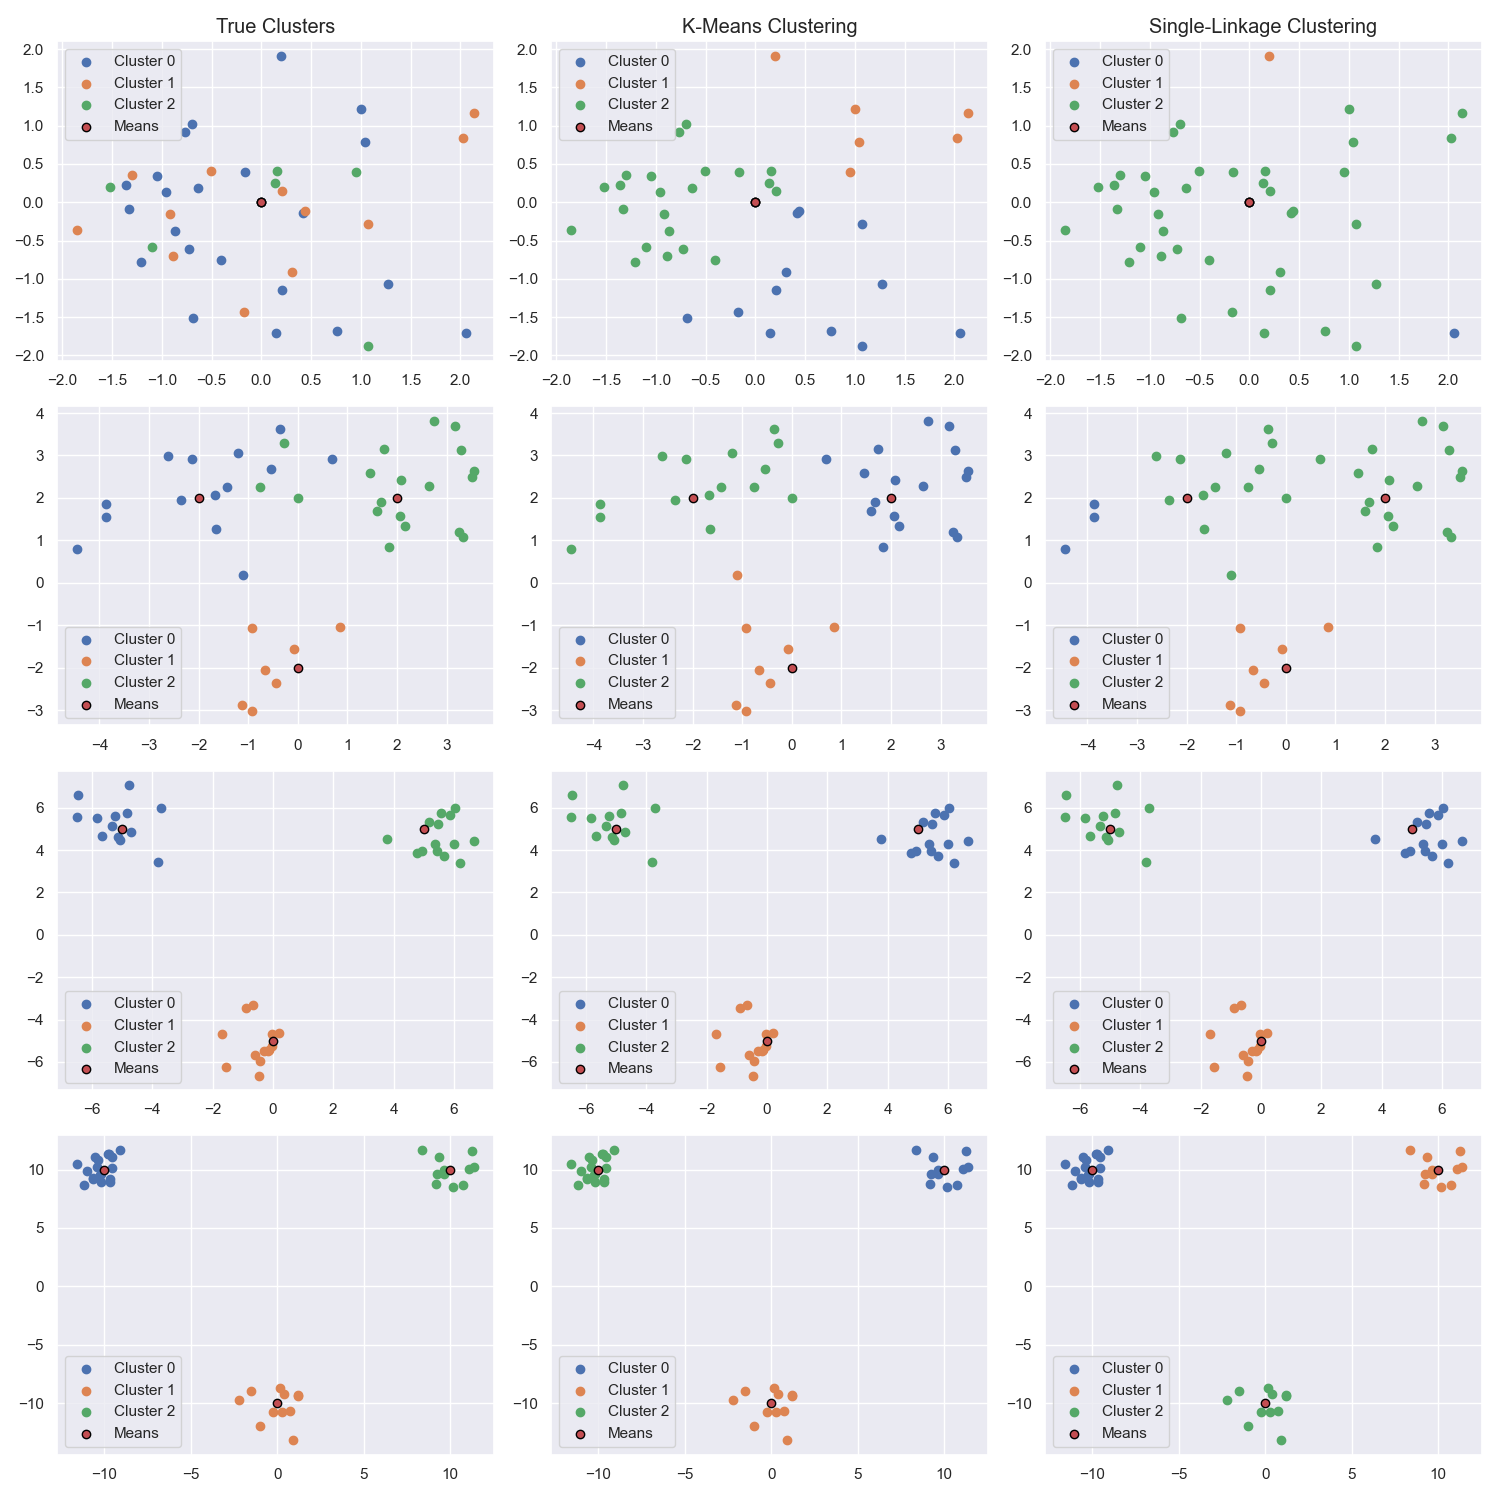
\includegraphics[width=0.99\linewidth]{images/q1/kmeans_singlelinkage.png}
        \caption{$k$-means vs single-linkage clustering on $3$ Gaussians with means at different distances}
    \end{figure}
    \pagebreak

\section[short]{$k$-means Clustering With Noise}

    \subsection[short]{Gaussian Noise}

        I added Gaussian noise $\mathcal{N}(0, \sigma^2)$ to my data $\mathbf{X}$. I plot the true clusters and set $\sigma^2$ to the following values: $0, 0.5, 1, 2, 5$. When $\sigma^2=0$, $k$-means performs well, correctly clustering nearly all the data points. However, as the noise increases, $k$-means becomes less and less accurate. Due to the random intialization of the means, $k$-means is very sensitive to noise -- this is why multiple runs of $k$-means is often recomemended.
        
        \begin{figure}[ht]
            \label{fig:kmeans_gaussian_noise}
                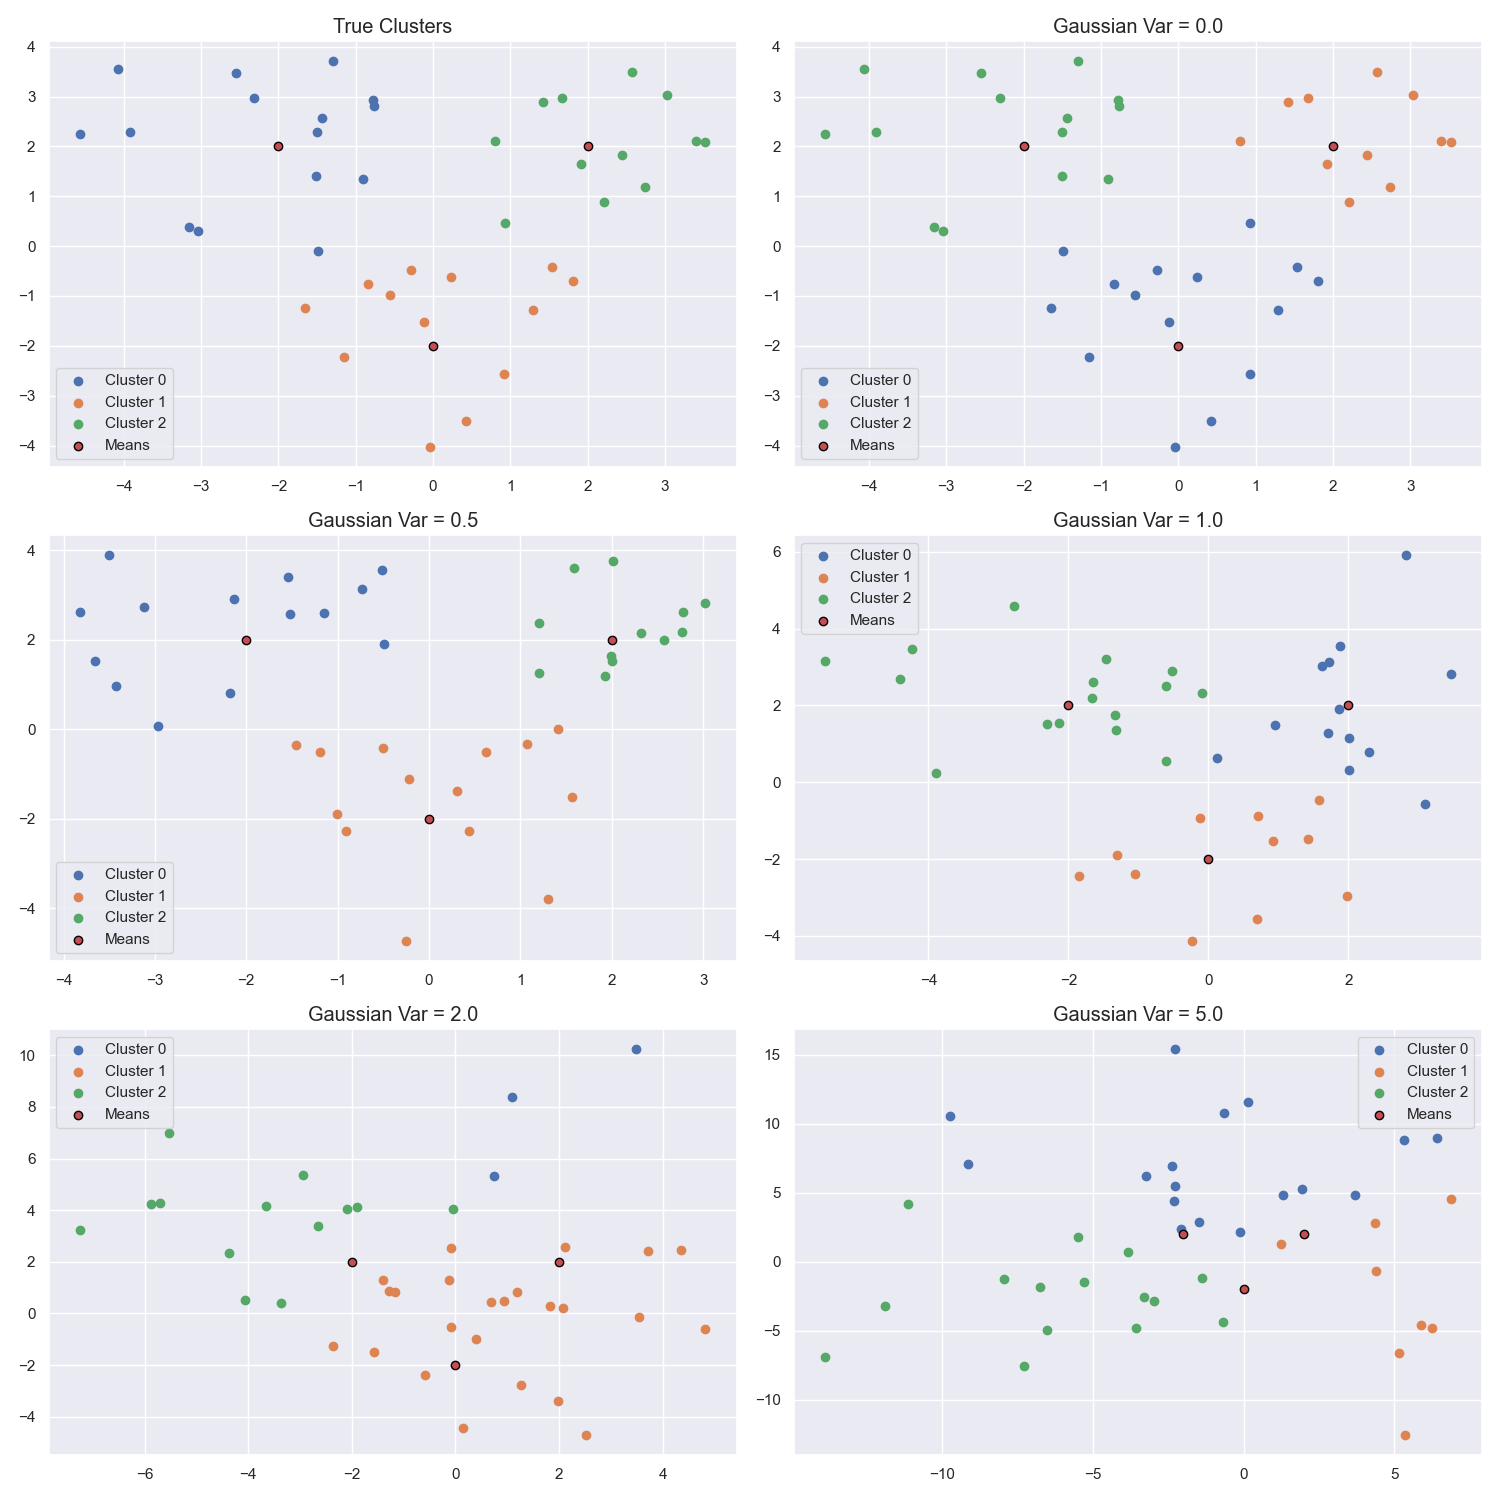
\includegraphics[width=0.99\linewidth]{images/q2/gaussian_noise.png}
                \caption{$k$-means with increasing amounts of Gaussian noise}
            \end{figure}
            \pagebreak

    \subsection[short]{Adversarial Noise}

        Adversial noise in single-linkage clustering can be used to create a "bridge" between two clusters that are otherwise far apart. In $k$-means clustering, for a given cluster-center initialization, adversarial points may also sometimes create a "bridge" that slowly shifts the cluster center towards the adversarial point as the algorithm converges. However, this problem is much severe than in the case of single-linkage clustering. Furthermore, adversarial noise can be used to place all $L$ data points into their own cluster which $k$-means would miss. Lastly, adversarial noise can challenge $k$-means clustering by creating a uniform grid of points, if $|L|$ is sufficiently large enough; this would rendure the entire clustering procedure useless and unusable.

\section[short]{Hierarchial $k$-Means and $k$-Medians}

        One can make a hierarchial version of $k$-means or $k$-medians as $k$ varies. However, there are many challenges that arise from the non-deterministic initialization of these algorithms. If there was a fixed rule, this would alleviate such problems.
        
        Nonetheless, there are interesting extensions that can create a form of hierarchial $k$-means or $k$-median algorithms -- I will elaborate upon one such way. Let there be $k$ desired clusters and $n$ data points $x_1 \ldots x_n$.

        Hierarchial clustering e.g. single-linkage clustering suffers from expenstive computational overhead. If one knows the general range of desired clusters, i.e. $k=[4,10]$, hierarchial clustering begins from $k=n$, where $n$ can be tens or hundreds of thousands of data points. Instead, one can run $k$-means or $k$-medians with $k=10$ and merge the nearest clusters as per single-linkage clustering. This would allow one to more efficeintly create a dendrogram with only $k=[4,10]$, for example. However, to ensure robustness, one would want to initialize $k$-means and $k$-medians multiple times and compare the results.

\section[short]{Clustering Data With $k$-means and \\ Single-Linkage Clustering}

    \subsection[short]{Clustering Dataset 1}

        When I cluster the ps1-clustering.txt dataset with both $k$-means and single-linkage clustering, there appear to be $7$ clusters. This is confirmed by the figure \ref{fig:dataset1} below. Single-linkage clustering perform better on this dataset, better and more easily separating the clusters, especially the center cluster. This occurs because $k$-means while only identify this as its own cluster if one of the cluster centers happened to be intialized to this center cluster. However, single-linkage clustering is not affected by this problem.

        \begin{figure}[]
            \label{fig:dataset1}
            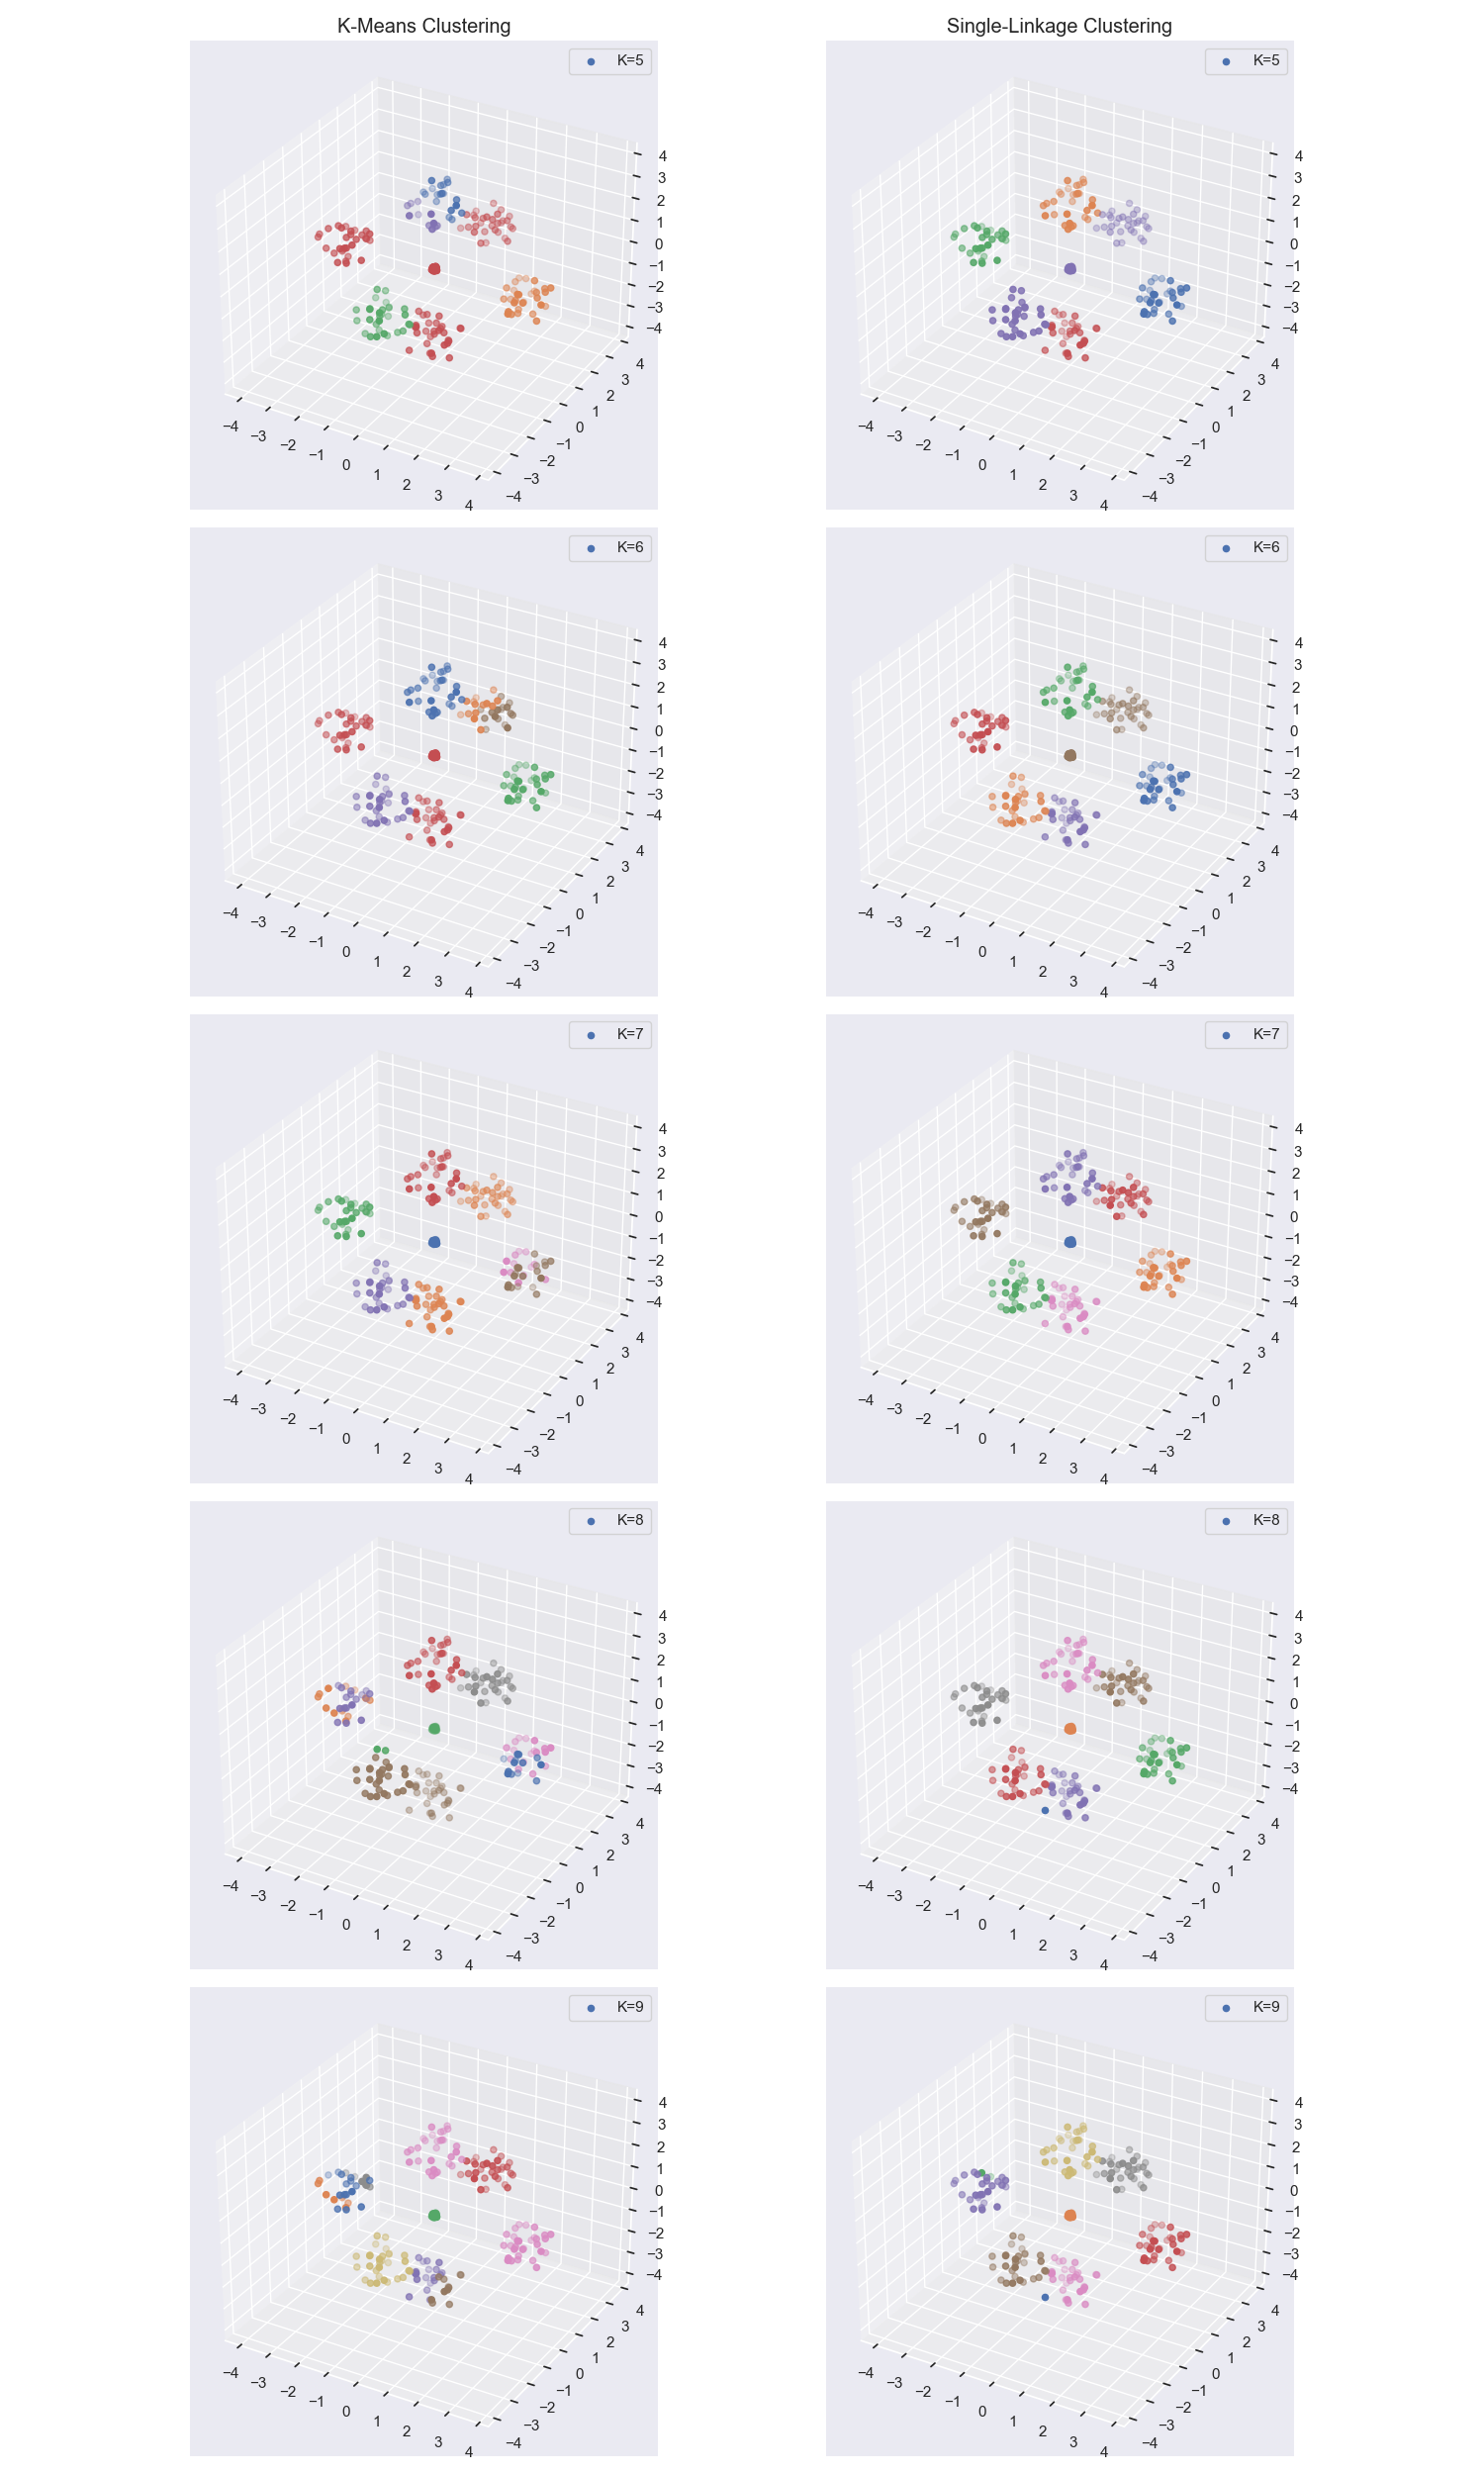
\includegraphics[width=0.90\linewidth]{images/q4/clustering-dataset1.png}
            \caption{$k$-means and single-linkage clustering on ps1-clustering.txt}
        \end{figure}
        \newpage

    \subsection[short]{Clustering Dataset 2}

        This dataset appears to have no real structure to it -- it is unclear how many clusters exist. However, single-linkage clustering often collapses into one cluster. $k$-means performs somewhat better, but it is not clear how many clusters to choose. This can be seen in the figure below \ref{fig:dataset2} which clusters according to both $k$-means and single-linkage clutsering for a variety of cluster values $k$ to little success.

        An interesting extension would be to measure the silhouette or Calinski-Harabasz score for each $k$ and choose the $k$ with the highest value score.

        \begin{figure}[]
            \label{fig:dataset2}
            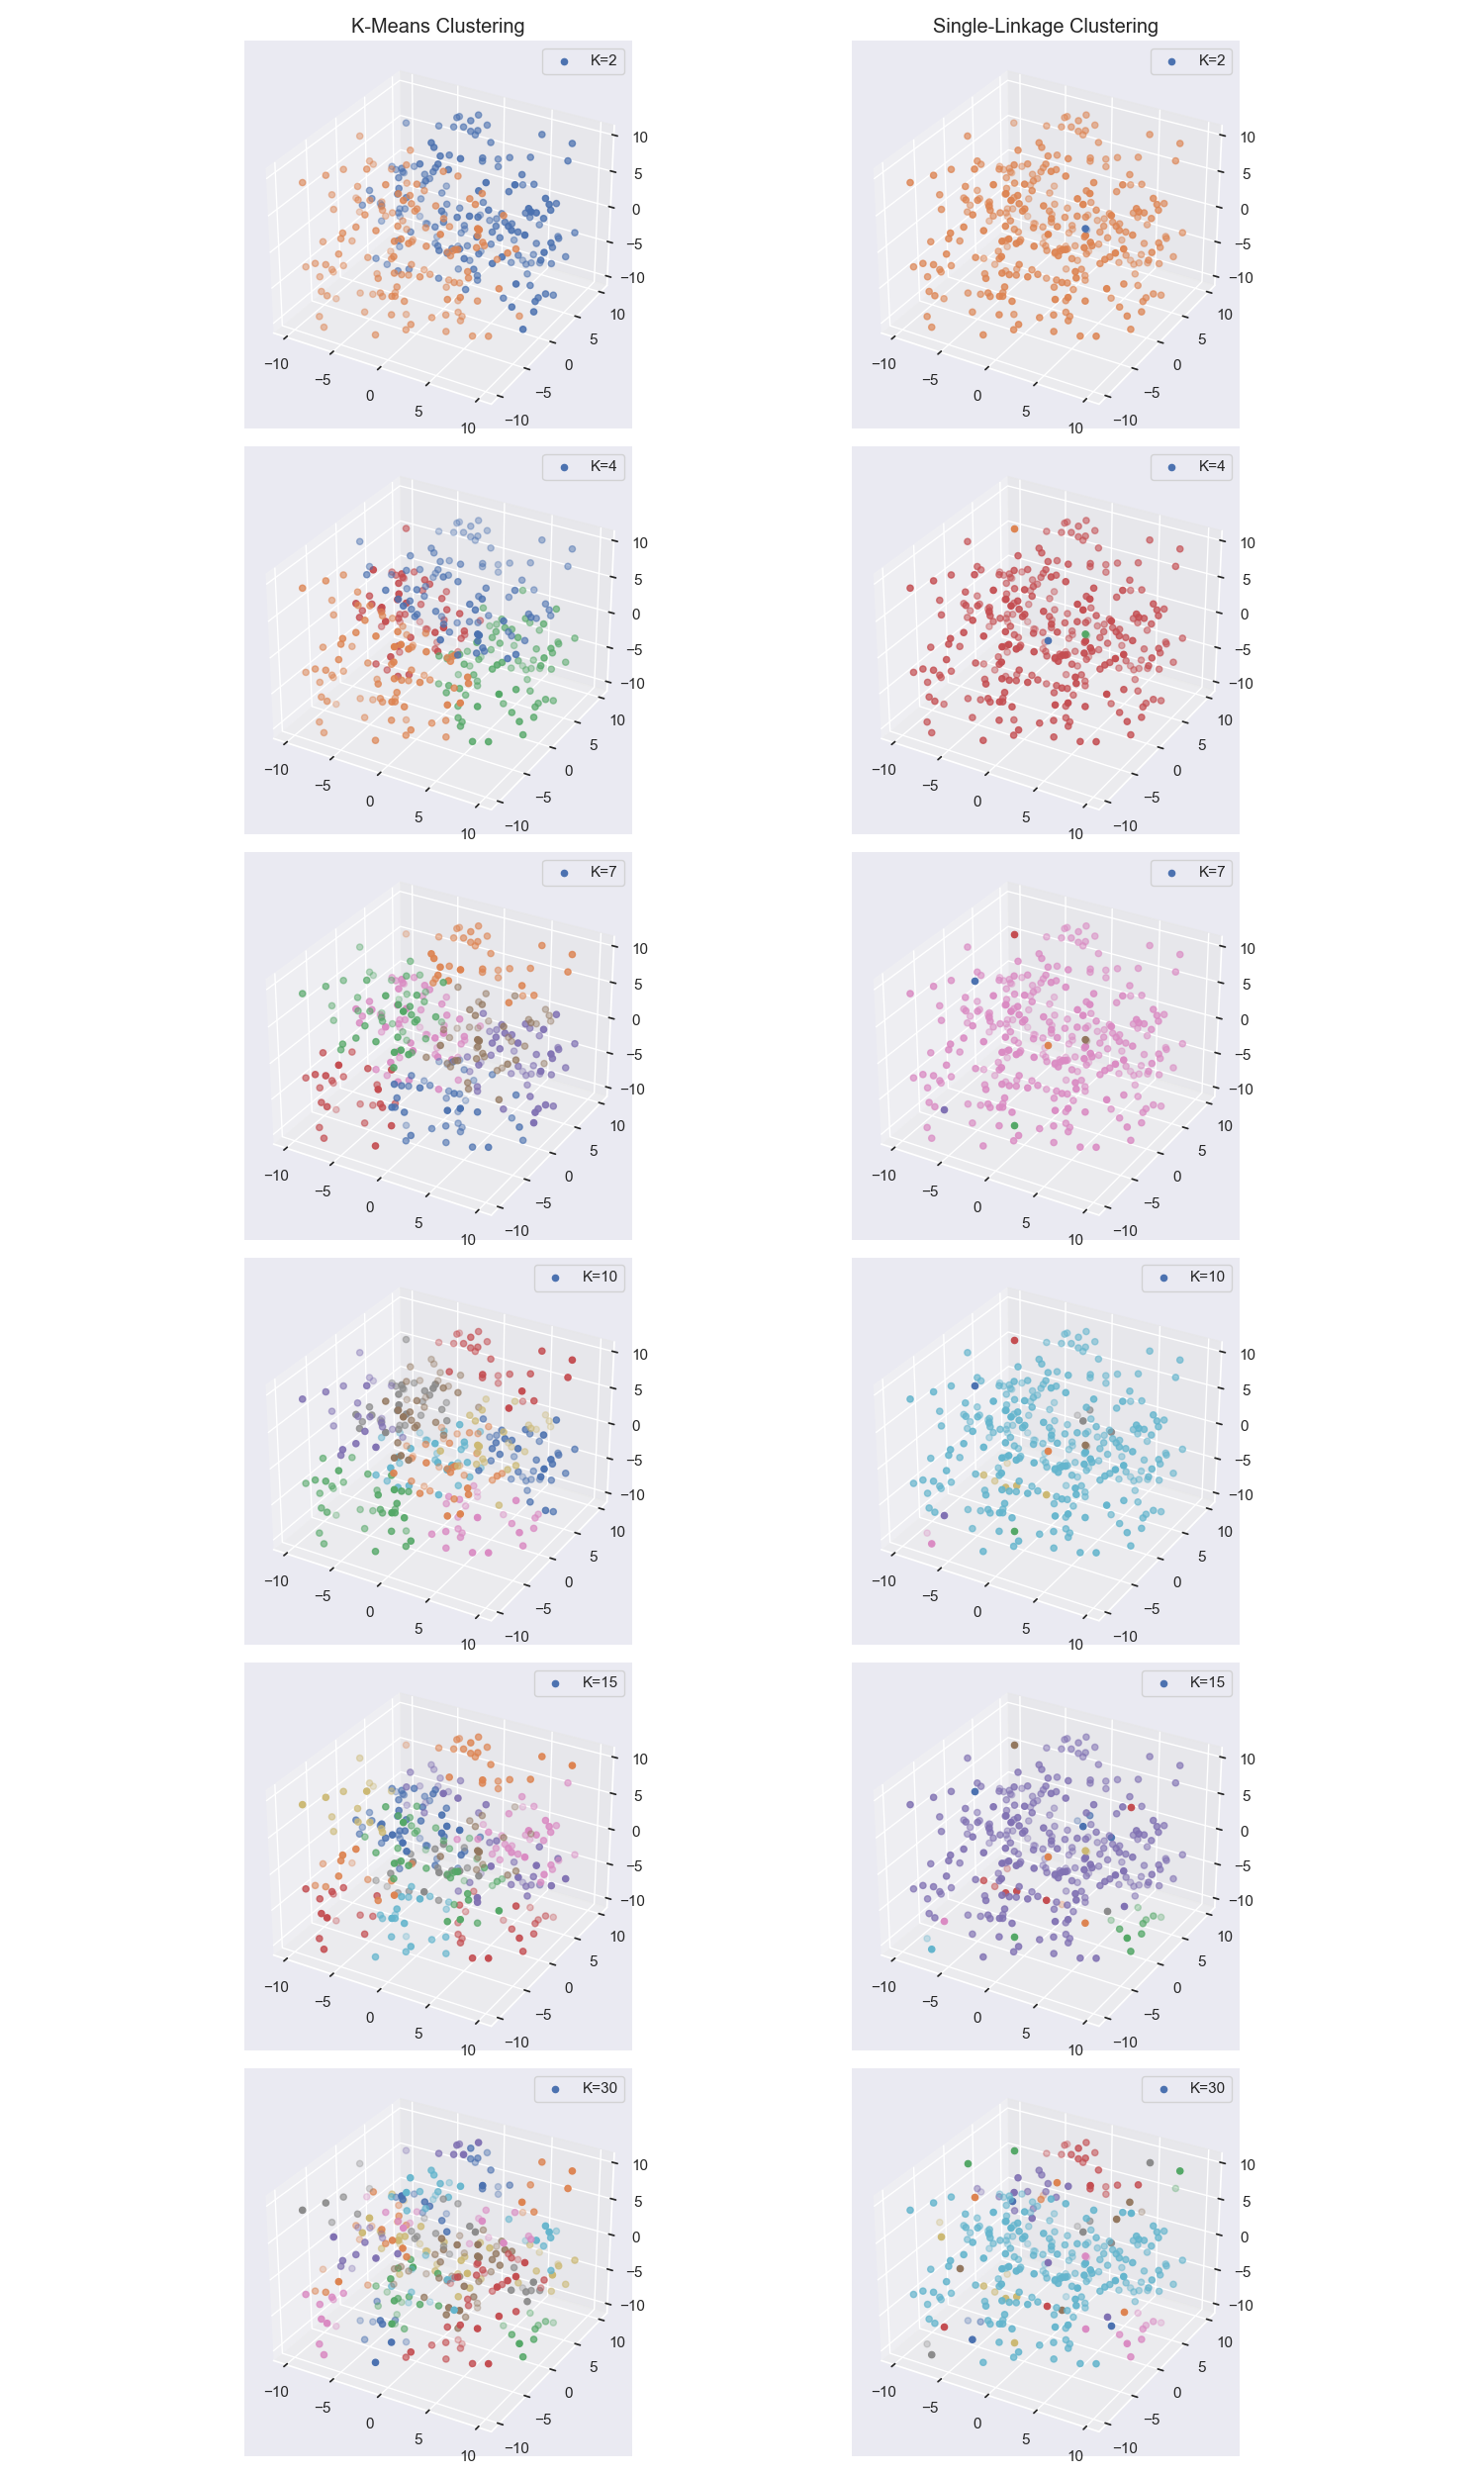
\includegraphics[width=0.90\linewidth]{images/q4/clustering-dataset2.png}
            \caption{$k$-means and single-linkage clustering on ps1-data.txt}
        \end{figure}
        \newpage

\section[short]{$k$-means Clustering Does Not Satisfy Consistency}

    This question invokes Jon Kleinberg's famous 2002 paper, An Impossibility Theorem for Clustering. In it, he proves that no clustering algorithm can satisfy the following three properties: scale-invariance, richness, and consistency.

    This question touches upon the consistency property, applied to the $k$-means algorithm: "suppose that the clustering $\Gamma$ arises from the distance function $d$. If we now produce $d ^ \prime$ by reducing distances within the clusters and enlarging distance between the clusters then the same clustering $\Gamma$ should arise from $d ^ \prime$". 

    $k$-means trivially does not satisfy the consistency property, as do all centroid-based methods. For a simple example, let $k=2$ and consider a set of points $S$. Divide $S$ into two subsets, $X$ with $m$ data points and $Y$ with $m \gamma$ data points for small $\gamma > 0$. Let the distance between points in $X$ be $r$ and the distance between points in $Y$ be some small $\epsilon > 0$. Then let the distance between clusters $X$ and $Y$ be $r + \delta$ for some small $delta > 0$. Then some initialization of $k$-means would select a point from $X$ and $Y$ which would result in the (true) clusters $X$ and $Y$. However, consider splitting up $X$ into sets $X_0, X_1$ with equal number of points. Then reduce the distance between points in $X_0$ to $r ^ \prime < r$ and similarly reduce the distance between points in $X_1$ to $r ^ \prime < r$. This changes the optimal choice of centroids to be points in $X_0$ and $X_1$ which would result in the (false) clusters $X_0$ and $X_1$.

    A similar type of intuition is captured in the figure below \ref{fig:consistency_violation}.

    \begin{figure}[ht]
        \label{fig:consistency_violation}
        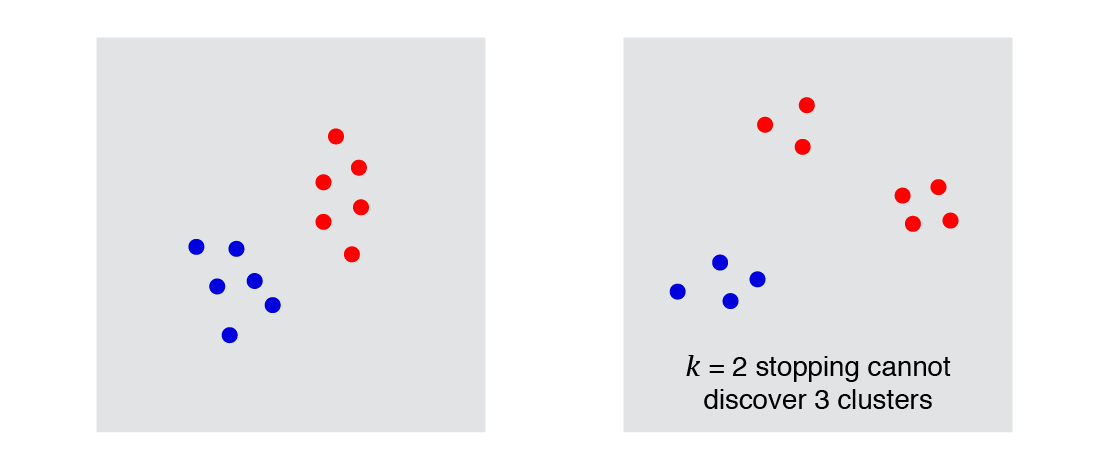
\includegraphics[width=0.90\linewidth]{images/q5/k-means_concistency.png}
        \caption{$k$-means unable to satisfy clustering consistency}
    \end{figure}
    \pagebreak

\section[short]{Clustering Annuli With $k$-means and Spectral Clustering}

    Unsuprinsingly, spectral clustering performs much better than $k$-means on the annuli dataset. This is because $k$-means uses Euclidean distance while spectral-clustering creates a graph which captures local notions of distance. Thus, $k$-means will compute points in two different annuli as being much closer together than the spectral clustering algorithm. This can be seen in the figure below \ref{fig:annuli}.

    \begin{figure}[ht]
        \label{fig:annuli}
        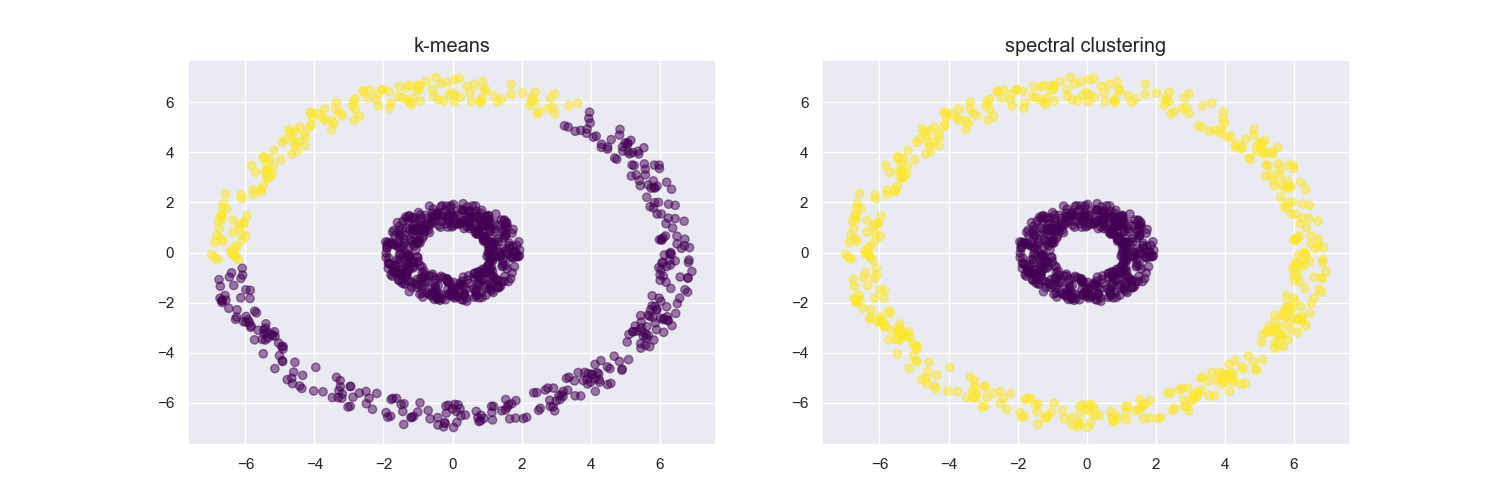
\includegraphics[width=0.90\linewidth]{images/q6/k-means_vs_spectral_clustering.png}
        \caption{$k$-means vs spectral clustering on annuli data}
    \end{figure}
    \pagebreak

\section[short]{Spectral Clustering: RBF Kernel vs \\ K-Nearest Neighbors}

    I ran spectral clustering, constructing graph weights both with Gaussian / radial basis function (RBF) kernel and selecting K nearest neighbors ($k$-NN). When creating a graph with RBF, I ensured the weight matrix was symmetric: if $x$ is a nearest neighbor of $y$, I made $y$ a nearest neighbor of $x$. Furthermore, I selected the RBF kernel parameter as $\sigma = 1$ and the $K$ nearest neighbor as $num neighbors = 7$. 

    I first compared RBF and $k$-NN on the concentric annuli. I set the radi of the first annuli to $r_{\textrm{min}}^1 = 1, r_{\textrm{max}}^1 = 2$ and set the radi of the second annuli to $r_{\textrm{min}}^2 = 5, r_{\textrm{max}}^2 = 6$. I generated $500$ points for each annuli. When there is no noise, both spectral clustering methods perform well, succesfully clustering the data into clusters. However, when I add Gaussian noise with variance of $0.5$, the RBF kernel fails while $k$-NN does not. This occurs because the noise jiggles data points in the two different annuli closer together, thus giving them more weight according to the RBF kernel function. However, the $k$-NN method does not suffer from this problem because it only considers the $k$ nearest neighbors.

    I then compared RBF and $k$-NN on a mixture of $1000$ datapoints sampled from $3$ Gaussians. These Gaussians have a variance of $1$ and means as follows:
    
    \begin{align*}
        \mu_1 = \begin{bmatrix} 0 \\ 0 \end{bmatrix} \qquad \mu_2 = \begin{bmatrix} 5 \\ 5 \end{bmatrix} \qquad \mu_3 = \begin{bmatrix} 8 \\ -4 \end{bmatrix}
    \end{align*}

    Again, both spectral clustering methods perform well when there is no noise. However, when I add Gaussian noise with variance of $2$, the RBF kernel fails while $k$-NN does not. This occurs because the noise jiggles data points in the two different Gaussians closer together, thus giving them more weight according to the RBF kernel function. However, the $k$-NN method does not suffer from this problem because it only considers the $k$ nearest neighbors.

    Ultimately, I conclude that the $k$-NN method is more robust to noise when clusters are close together.

    \begin{figure}[ht]
        \label{fig:rbf_vs_knn}
        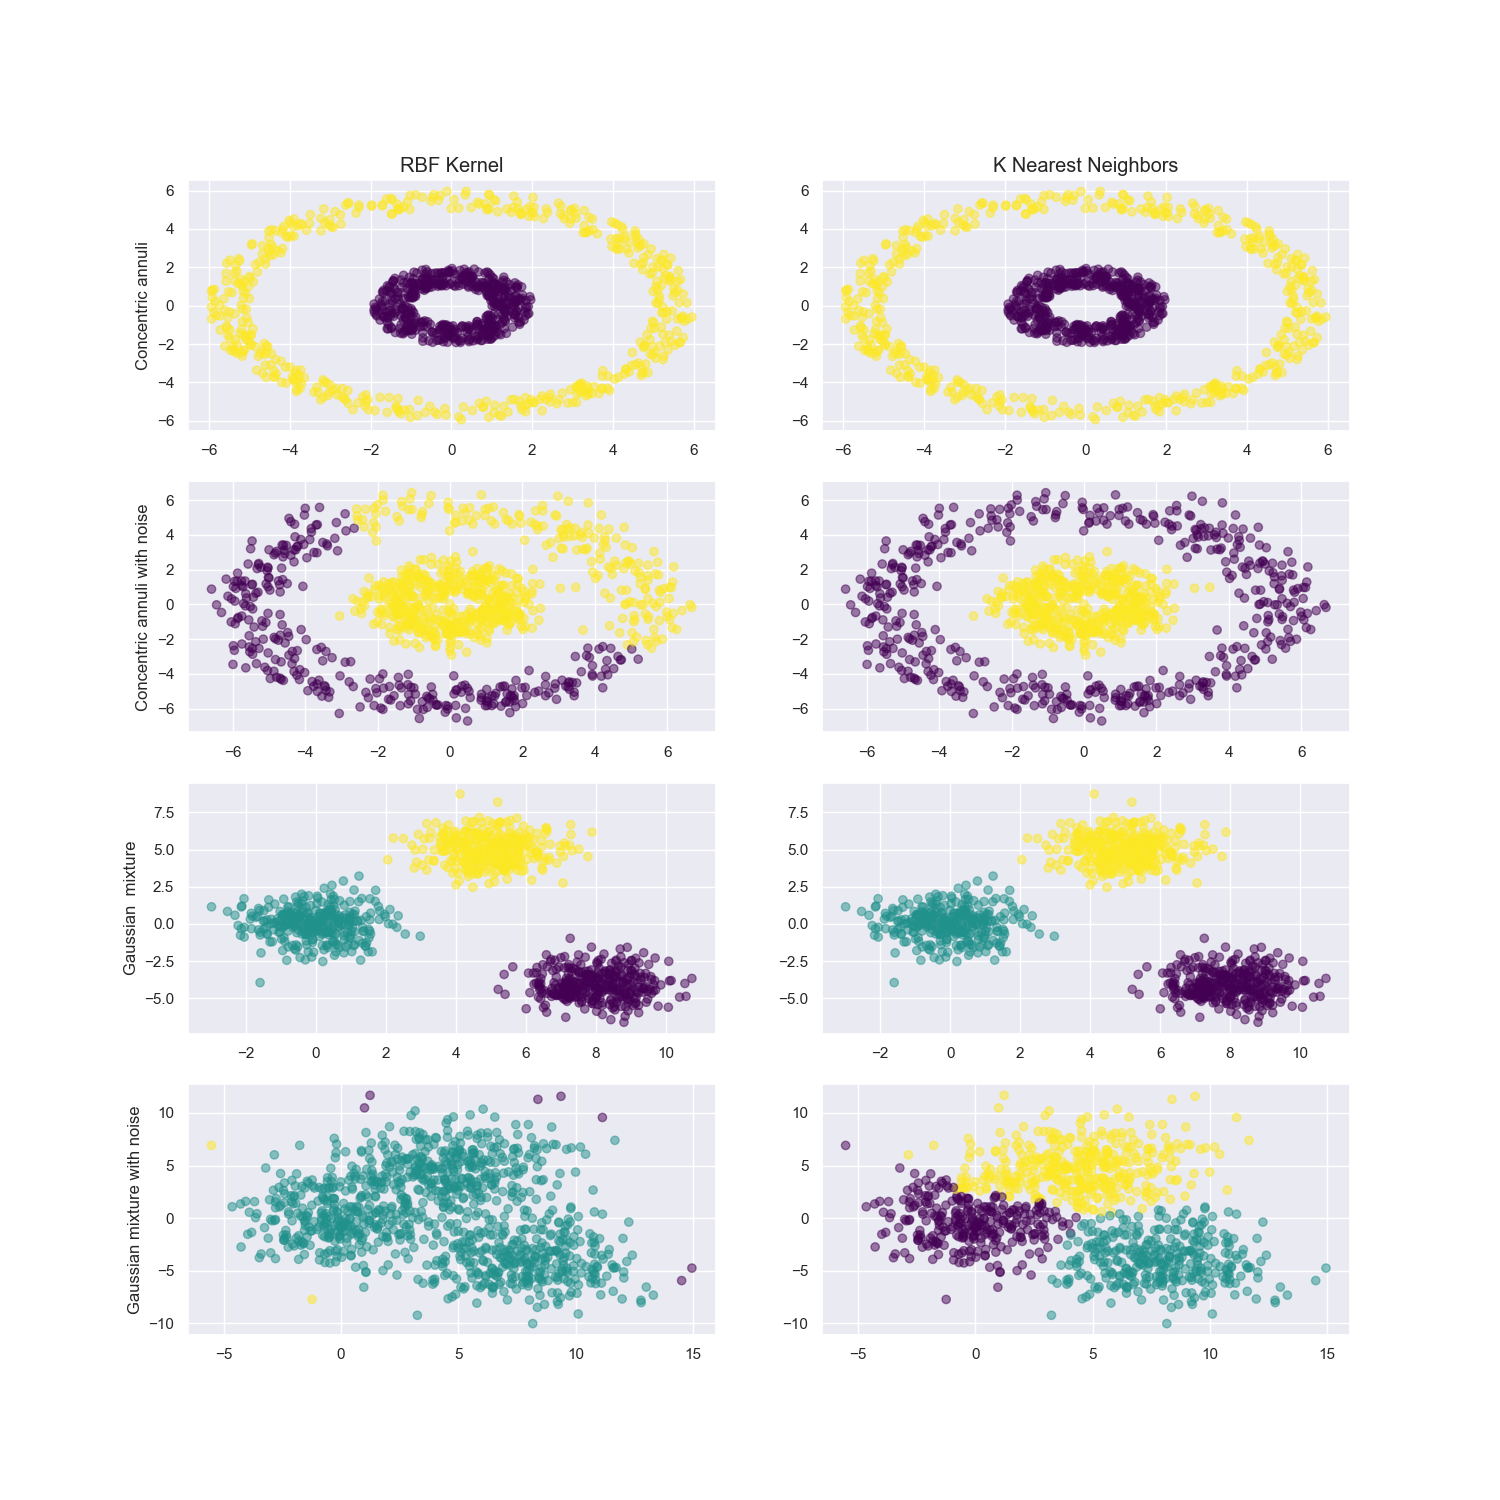
\includegraphics[width=0.99\linewidth]{images/q7/spectral_clustering:_rbf_vs_knn.png}
        \caption{Spectral clustering with RBF kernel vs $k$-NN}
    \end{figure}
    \pagebreak

\end{document}